\documentclass[10pt]{article}
\usepackage{graphicx}
\usepackage{amsmath}
\usepackage{float}
\usepackage{subcaption}
\usepackage[margin=1in]{geometry}


\begin{document}
\pagenumbering{gobble}
\begingroup  
  \centering
  \large Fast \& Sparse Learning with Hierarchical Concept Training\\[1em]
  \small{Andrew Lampinen* (lampinen@stanford.edu, Department of Psychology, Stanford University),\\ James McClelland (mclelland@stanford.edu, Department of Psychollogy, Stanford University)}\par
\endgroup
\vspace{10pt}
The end-to-end training on large data sets that is customary for neural networks is very unlike the way that adult humans learn tasks. Human learning is often rapid, and successful even with sparse data sets. In part, this is likely because humans can break problems down into successive steps, and can integrate previously learned concepts into their understanding. Work on curriculum learning has shown that learning in neural networks can be facilitated by teaching intermediate steps of the task (G{\"{u}l\c{c}ehre \& Bengio, 2013). Here, we suggest that even if the task is easily learnable in general, the technique of teaching intermediate steps can lead to much better performance on sparse data sets, and faster learning on larger data sets.\par
We demonstrate this by teaching networks the rules to Conway's Game of Life: a square with four or more neighbors dies from overcrowding, and one with fewer than two neighbors dies from loneliness, a live square with two or three neighbors lives, and a dead square with three neighbors becomes live. Calculating the life of a square can be decomposed into two separate steps: First, evaluating the current life of a unit and the number of its living neighbors, and second, computing its life at the subsequent time-step from these values. This can be seen as a task of learning a mapping from 3 x 3 binary arrays (representing the initial state) to a single binary value (representing the life of the central unit at the subsequent time step). Since there are 512 possible input arrays, we trained on $n$ of them (randomly selected), and tested on the held out $512-n$, while varying $n$. We trained the hierarchical network by training a single-layer (ReLU) network to extract number of neighbors and life of the central square from the problem, and simultaneously training a single hidden-layer (tanh) network to compute the life value at the next time step from the number of neighbors and the life value at the previous time step. (We trained the second network off the output values produced by the first, training off the perfect values did not significantly alter the results.) We compared the hierarchically trained network to a variety of standard neural networks (two hidden layers, first ReLU, second tanh, to imitate the structure of the hierarchical, and then two networks with one of the two hidden layers removed). These were trained with standard procedures on the full task. (See Figure \ref{networkdiagram} for a comparison of our network to the two hidden layer standard network.)\par
We demonstrated that the hierarchical network is able to learn from much sparser datasets than the standard networks (see Figure \ref{n64figure} for an plot of error rate for the different networks, averaged across 100 trials, with $n = 64$ training examples, the average error rates do not quite reach zero because with $n = 64$, even the hierarchical network was not always successful at learning the task, but it succeeded in over 80\% of the cases). Furthermore, even with datasets sufficient for the standard networks to learn, the hierarchical networks learned the task much more rapidly (see Figure \ref{n256figure}). We conclude that hierarchically trained networks can offer benefits for sparse learning, and for rapid learning even on large data sets, and that alternative approaches such as these may lead to more human-like learning from neural networks.
\begin{figure}[H]
    \centering
    \begin{subfigure}[c]{0.35\textwidth}
	\centering
	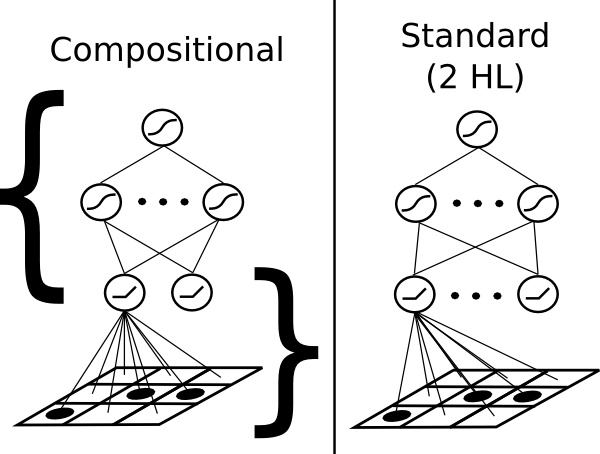
\includegraphics[width=\textwidth]{figures/hierarchical_NN_abstract_figure.png}
	\caption{Network comparison (brackets in hierarchical network denote the sub-networks we trained.)}
	\label{networkdiagram}
    \end{subfigure}
    \begin{subfigure}[c]{0.3\textwidth}
	\centering
	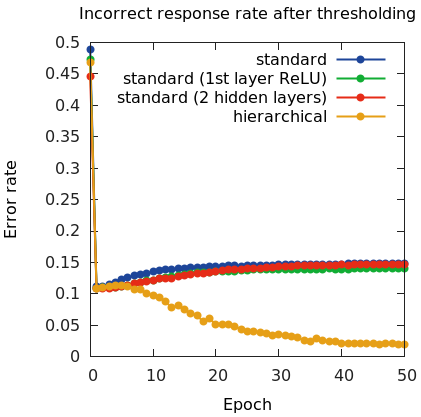
\includegraphics[width=\textwidth]{figures/n64figure.png}
	\caption{Error rates for $n = 64$}
	\label{n64figure}
    \end{subfigure}
    \begin{subfigure}[c]{0.3\textwidth}
	\centering
	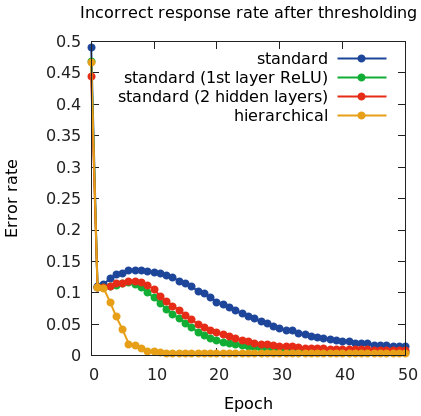
\includegraphics[width=\textwidth]{figures/n256figure.png}
	\caption{Error rates for $n = 256$}
	\label{n256figure}
    \end{subfigure}
    \caption{Network comparison \& results}
\end{figure}

\end{document}
